\chapter{Aggregated Set Membership Proofs}
\label{ch:generalAgg}
It is of high importance to keep the computational complexity for the verification of set membership proofs small, 
%The computational complexity for verification of set membership proofs is important to keep small,
 specially in applications where one verifier validates multiple provers. If set membership proofs, which are proofs of the statement:
\begin{align*}
    \{(g,h\in\mathds{G},C\in\mathds{G};x,R\in\mathds{F})\::\:C= g^x h^R \wedge x \in \Phi\},
\end{align*}
are used to verify multiple provers then the verifier would have to verify each prover individually. This leads to that the computational complexity for verification grows linearly in the number of provers and the verification algorithm quickly becomes a bottleneck in application where many provers participates. 

This motivates the question if set membership proofs can be aggregated, and thereby decreasing the computations required to verify multiple provers. 

A definition of aggregated set membership proofs is presented  in Definition \ref{def:GeneralAggregation}. An aggregated set membership proof is defined to be a  $5$-tuple of PPT algorithms,  (\textbf{SetUp}, \textbf{Prove}, \textbf{Aggregate}, \textbf{CalculateChallanges}, \textbf{Verify} ).


\vspace{10pt}
\begin{Mydef}[\textbf{Aggregated set membership proofs}]
\label{def:GeneralAggregation}
Aggregated set membership proofs are a zero-knowledge proof of the statement:
\begin{equation}
\begin{aligned} 
\label{eq:SMagg_statement}
    \big\{(g,h\in\mathds{G},\{C_i\}_{i\in\mathcal{S}}\in\mathds{G}^n;\:\{x_i\}_{i\in\mathcal{S}},\{R_i\}_{i\in\mathcal{S}}\in\mathds{F}^n)\:: 
\: &C=\prod_{i\in\mathcal{S}}C_i 
\\
 &\wedge \prod_{i\in\mathcal{S}}C_i  =   g^{\sum_{i\in\mathcal{S}}x_i} h^{\sum_{i\in\mathcal{S}}R_i} 
 \\
 &\wedge x_i \in \Phi \: \forall i\in\mathcal{S} \big\}.
\end{aligned}
\end{equation}
Where $C_i$ is a Pedersen commitment to the secret $x_i\in\mathds{F}$ and $R_i \in_R\mathds{F}$ are chosen at random, for all $i\in\mathcal{S}$.  

The statement implies that after successfully having performed an aggregated set membership proof protocol, it is proved that the aggregated Pedersen commitment, $C$, is a product of the Pedersen commitment,$\{C_i\}_{i\in\mathcal{S}}$ and that for all $i\in\mathcal{S}$ $C_i$ is a Pedersen commitment to a secret $x_i$ belonging to the set $\Phi$.

A construction of aggregated set membership proofs is a $5$-tuple of PPT-algorithms (\textbf{SetUp}, \textbf{Prove}, \textbf{Aggregate}, \textbf{CalculateChallanges}, \textbf{Verify}).
\\
\begin{itemize}
  \item\textbf{SetUp $(1^\lambda, \Phi)\xrightarrow[]{}(pp,sk)$}\\
On the input $1^\lambda$, where $\lambda$ is the security parameter and the set $\Phi$ the algorithm outputs a secret key, $sk$, and public parameters, $pp$. 

\item\text{\textbf{Prove} $(pp,i,C_i,x_i,\Phi) \xrightarrow[]{} \Sigma_i$}\\
On the input, the public parameters $pp$, $i\in\mathcal{S}$ denoting the index of the prover $p_i$, a secret $x_i$ and a Pedersen commitment $C_i$ of the secret.  The algorithm outputs a polynomial time verifiable zero-knowledge proof of the statement in equation \eqref{eq:SM_statement}, denoted $\Sigma_i$.

\item \text{\textbf{Aggregate} $ (pp,\{\Sigma_i\}_{i\in\mathcal{S}} \xrightarrow[]{} \Sigma_a$} \\
Given a set of set membership proofs  $\{ \Sigma_{i}\}_{i\in\mathcal{S}}$ the algorithm aggregates the proofs into one zero-knowledge proof of the statement in equation \eqref{eq:SMagg_statement} denoted $\Sigma_a$. 

\item \text{ \textbf{CalculateChallenges} $(\{C_i\}_{\in\mathcal{S}},\{\sigma_i\}_{i\in\mathcal{S}} ) \xrightarrow[]{} \{c_i\}_{i\in\mathcal{S}}$ }\\\
On the input $\{\Sigma_i\}_{i\in\mathcal{S}}$ the algorithm computes and outputs the challenges  $c_i = Hash(\Sigma_i)$ for all $i\in\mathcal{S}$.

\item\text{\textbf{Verify} $(pp, \Sigma_a, \{C_i\}_{i\in\mathcal{S}},\{c_i\}_{i\in\mathcal{S}}) \xrightarrow[]{} \{0,1\}$} \\
On input the aggregated set membership proof public parameters, $pp$, aggregated proof, $\Sigma_a$, the Pedersen commitments, $\{C_i\}_{i\in\mathcal{S}}$, and challenges ,$\{c_i\}_{i\in\mathcal{S}}$, the algorithm outputs either $1$ or $0$. 
\end{itemize}

\end{Mydef}
\vspace{10pt}

Aggregated set membership proofs consist of the following parties: provers, an aggregator and a verifier. A schematic figure of the interaction between the parties is seen in Figure \ref{fig:gen_workflow}. The provers, a group of many individual provers, individually run the algorithm \textbf{Prove} and publishes the computed proof. The aggregating party retrieves all proofs, runs the algorithm \textbf{Aggregate} and publishes the aggregated proof. Finally, the verifier validates the aggregated proof by running the algorithm \textbf{Verify}.  The aggregation can be split between multiple parties implying there are many aggregators, this is discussed more in the next chapter. The algorithms \textbf{SetUp} and \textbf{CalculateChallenges} is either performed by the verifier or by an independent trusted party.

 \begin{figure}
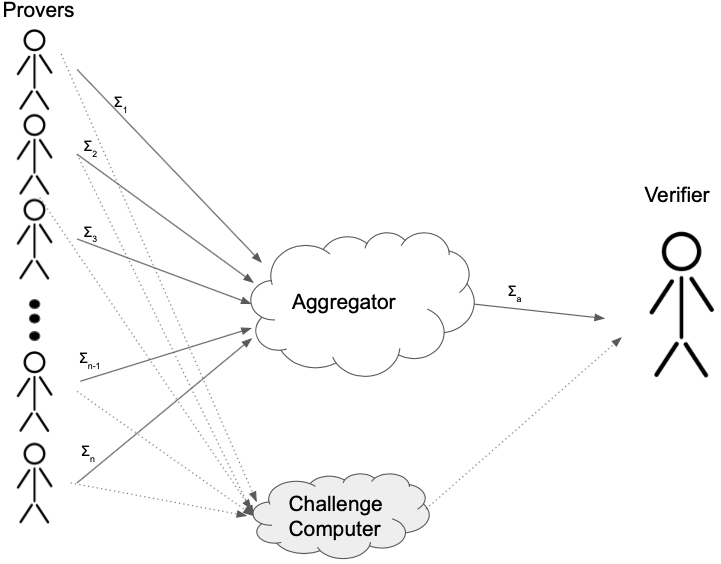
\includegraphics[width=\linewidth]{./figure/oneagg.png}
\caption{Schematic figure of the interaction between Provers, Aggregator and Verifier in aggregated set membership proofs. }
\label{fig:gen_workflow}
\end{figure} 


%TODO fix can this be here?  ONLY range proofs
%A remark is that to aggregate the commitments $C_i, \: i\in\mathcal{S}$ into $C = \prod_{i\in\mathcal{S}} Ci_i$. Then constructing  a range proof that the aggregated commitment $C = g^{\sum_{i=1}^n x_i}$ belongs to the range  $[n\cdot a,n\cdot b]$, does not prove that $x_i \in [a,b]$ for all $i \in\mathcal{N}$. In other word is does not satisfy the verification property in Theorem \ref{thm:VAHSS_RP_CSV}. The value $y=\sum_{i=1}^n x_i$ is publicly known so to construct a zero-knowledge range proof for $y $ provides no new information and given that $y\in [n\cdot a,n\cdot b]$ does not imply $x_i\in [a,b]$ for all $i\in\mathcal{N}$. 


The algorithms of aggregated set membership proofs, presented in Definition \ref{def:GeneralAggregation}, should fulfil the below completeness, soundness and zero-knowledge requirements:
\begin{itemize}
\item \textbf{Completeness} Given a witness $\Sigma_i$ satisfying the instance $x_i\in\Phi$, where $C_i$ is a Pedersen commitment of $x_i$, for all $i\in\mathcal{S}$, it should hold that
\\
 \texttt{Verify}$($\texttt{Aggregate}$(\{$\texttt{Prove}$(pp,i,C_i,\Phi)\}_{i\in\mathcal{S}}) )= 1$. 
\item \textbf{Soundness} If for any $i\in\mathcal{S}$ the  witness $\Sigma_i$ does not satisfy the  instance $x_i\notin\Phi$, then the probability  Prob$[ $\texttt{Verify}$($\texttt{Aggregate}$(\{$\texttt{Prove}$(pp,i,C_i,\Phi)\}_{i\in\mathcal{S}}) ) = 1] < \varepsilon$, for a sufficiently small $\varepsilon$. 
\item  \textbf{Zero-knowledge} 
A proof system is \textit{honest verifier zero-knowledge} if there exists a PPT algorithm \texttt{Simulator} having access to the same input as the algorithms \texttt{Verify} and \texttt{Aggregate} but not the provers input, such that output from the \texttt{Simulator} and \texttt{Prove} is indistinguishable, i.e have the same distribution given that $x\in\Phi$.  
\end{itemize}

These requirements can be seen as a modification of the requirements given in Definition \ref{def:ZKP} to aggregated set membership proof. Note that the zero-knowledge property should hold for the provers, not the aggregation.



%\subsection*{Many aggregation}
%TODO Decise if use
